\section{Methodology}
\subsection{Description}
\noindent\fbox{
	\parbox{\textwidth}{
		\textbf{1.} Define a methodology$^1$ using SysML/UML diagrams for the development of your system. Specify SysML/UML diagrams that need to be made in the different phases of the project. Make a short description of each design phases and the SysML/UML diagrams and profiles you decide to use in the methodology. Remember to use references to the papers you have use as inspiration for your work. Decide on an UML$^2$ tool.
	}
}\citepawesome{Bjerge2017}{1}


\subsection{SysML}
In this project SysML standard will be used to describe the system as a whole, but also to help describe core functionality down to the wire. The usage of SysML standard is decided upon because of the structural approach to the analysis. To ensure cohesion throughout the usage of SysML and UML, the \textit{"A Practical Guide to SysML: The Systems Modeling Language"}\cite{Friedenthal2014} document will be used. This report will follow a Top-Down approach as stated below:

\begin{itemize}
	\item Analyzing the Problem
	\item Model Organization
	\item Operation
	\begin{itemize}
		\item Use Cases
		\item Requirements
	\end{itemize}
	\item Structure
	\begin{itemize}
		\item Block Definition Diagram (bdd)
		\item Internal Block Diagram (ibd)
	\end{itemize}
	\item Behavior
	\begin{itemize}
		\item Sequence Diagram (sd)
		\item Activity Diagram (act)
		\item State Machine Diagram (smd)
	\end{itemize}
\end{itemize}


Microsoft Visio, with the included stencil toolbox\citeawesome{Hruby2018}, and Visual Studio 2017 Enterprise will be used as UML tools.

\subsection{Analyzing the Problem}
To make a Domain Model we start by a analysis of the description on page \pageref{sc:problemdescription}. Here we find the following nouns in the text and then they can be used later to get a good cobbling between problem and models.

\textbf{This could be removed if it does not make sense}



\subsection{Model Organization}
To manage the complete model and sub-models of the full system, the package diagram\citepawesome{Friedenthal2014}{103} will be used. A package diagram is a system organization model of SysML standards. In this project the package diagram will be used to formulate and verify which diagrams and models are used as a methodology to describe the system of interest. Another effect the package diagram have on this project, is the organization structure it brings.\\

Multiple package diagrams are used to explain dependencies of components and sub-systems in a complex system. Since this project is of a smaller scale, only a single package diagram is needed. However this 

\subsection{Operation}
\blindtext

%==================== Fully Dressed Use Cases ====================

\subsubsection{Use Case Diagram} \label{sec:usecasediagrams}

\blindtext
%For alle Use Cases hvor brugeren navigerer i undermenuer af hovedmenuen, gælder det, at brugeren har mulighed for at gå et skridt tilbage ved at trykke på en ”tilbage knap”. Fremover ved benævningen ”Systemet er operationelt” menes, at systemet er tilsluttet strømforsyning og at alt fungerer samt at systemet er tilsluttet ethernet.

\begin{figure}[!h]
	\centering
	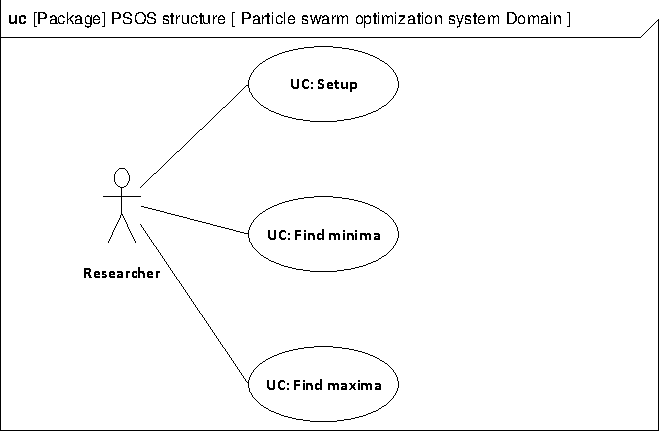
\includegraphics[width=0.8\linewidth]{diagram/uc_particle_swarm_optimization_system.pdf}
	\caption{Use Case Diagram of Particle Swarm Optimization}
	\label{fig:ucdiagram}
\end{figure}


%-------------------- UC1 --------------------
\begin{table}[h]
\begin{tabularx}{\textwidth}{| >{\raggedright\arraybackslash}p{3.3 cm} | >{\raggedright\arraybackslash}X |} \hline

\textbf{Name:} 						& UC1: Start\\ \hline
\textbf{Goal:}						&  \\ \hline
\textbf{Initering:}					&  \\ \hline
\textbf{Actor:} 					& User (primær) \\ \hline
\textbf{Reference:} 					& UC10: Monitorering, UC11: Regulering \\ \hline
\textbf{Number of simultaneous occurrences:} & Én \\ \hline
\textbf{Pre-condition:} 				& \\ \hline
\textbf{Result:}					&  \\ \hline
\textbf{Main scenario:}				& 

\begin{packed_enum}
\item allaa
\item allala
\item alllaa
	\begin{packed_item}\itemsep1pt \parskip0pt \parsep0pt
	\item {[}Ext 3.a : User does not press "Regulation".{]}
	\end{packed_item}
\item Systemet aktiverer UC11: Regulering.
\item UC1 afsluttes.
\end{packed_enum} \\ \hline
\textbf{extensions:}				&  
\textbf{{[}Ext 3.a :User selects only monitoring.{]}}
	\begin{packed_enum}\itemsep1pt \parskip0pt \parsep0pt
	\item The system continues at point. 5 in the main scenario.
	\end{packed_enum}
\\ \hline
\end{tabularx}
\caption{UC1: Start}
\label{tbl:uc1}
\end{table}
%-------------------- UC2 --------------------
\begin{table}[h]
	\begin{tabularx}{\textwidth}{| >{\raggedright\arraybackslash}p{3.3 cm} | >{\raggedright\arraybackslash}X |} \hline
		
		\textbf{Name:} 						& UC2: Find minima\\ \hline
		\textbf{Goal:}						& Find the minima of a function \\ \hline
		\textbf{Initering:}					& Researcher \\ \hline
		\textbf{Actor:} 					& Researcher (primary) \\ \hline
		\textbf{Reference:} 				& UC1: Setup \\ \hline
		\textbf{Number of simultaneous occurrences:} & One \\ \hline
		\textbf{Pre-condition:} 				& UC1 has been done \\ \hline
		\textbf{Result:}					& Found the minima of a function \\ \hline
		\textbf{Main scenario:}				& 
		
		\begin{packed_enum}
			\item allaa
			\item allala
			\item alllaa
			\begin{packed_item}\itemsep1pt \parskip0pt \parsep0pt
				\item {[}Ext 3.a : User does not press "Regulation".{]}
			\end{packed_item}
			\item Systemet aktiverer UC11: Regulering.
			\item UC1 afsluttes.
		\end{packed_enum} \\ \hline
		\textbf{extensions:}				&  
		\textbf{{[}Ext 3.a :User selects only monitoring.{]}}
		\begin{packed_enum}\itemsep1pt \parskip0pt \parsep0pt
			\item The system continues at point. 5 in the main scenario.
		\end{packed_enum}
		\\ \hline
	\end{tabularx}
\caption{UC2: Start}
\label{tbl:uc2}
\end{table}
%-------------------- UC3 --------------------
\begin{table}[h]
\begin{tabularx}{\textwidth}{| >{\raggedright\arraybackslash}p{3.3 cm} | >{\raggedright\arraybackslash}X |} \hline

\textbf{Navn:} 						& UC1: Start\\ \hline
\textbf{Mål:}						& At starte systemet helt eller delvist. \\ \hline
\textbf{Initering:}					& Bruger \\ \hline
\textbf{Aktører:} 					& Bruger (primær) \\ \hline
\textbf{Reference:} 					& UC10: Monitorering, UC11: Regulering \\ \hline
\textbf{Antal samtidige forekomster:} & Én \\ \hline
\textbf{Forudsætning:} 				& Systemet er stoppet helt, er operationelt og viser hovedmenuen.\\ \hline
\textbf{Resultat:}					& UC10: Monitorering og evt. UC11: Regulering er startet, systemet viser Hovedmenuen. \\ \hline
\textbf{Hovedscenarie:}				& 

\begin{packed_enum}
\item Bruger trykker på "Monitorering". 
\item System aktiverer UC10: Monitorering. 
\item Bruger trykker på "Regulering". 
	\begin{packed_item}\itemsep1pt \parskip0pt \parsep0pt
	\item {[}Ext 3.a : Bruger trykker ikke "Regulering".{]}
	\end{packed_item}
\item Systemet aktiverer UC11: Regulering.
\item UC1 afsluttes.
\end{packed_enum} \\ \hline
\textbf{Udvidelser:}				&  
\textbf{{[}Ext 3.a : Bruger vælger kun monitorering.{]}}
	\begin{packed_enum}\itemsep1pt \parskip0pt \parsep0pt
	\item Systemet fortsætter ved pkt. 5 i hovedscenariet.
	\end{packed_enum}
\\ \hline
\end{tabularx}
\caption{UC3: Start}
\label{tbl:uc3}
\end{table}

\subsubsection{Requirements}
\subsection{Structure}

\subsubsection{Block Definition Diagram}
The system consist of three parts, a random generator, an user interface and the particle swarm logic. on Figure \ref{fig:bdd} the block definition diagram can be seen with these three parts, as part of the overall Particle Swarm Optimization System.

\begin{figure}[!h]
	\centering
	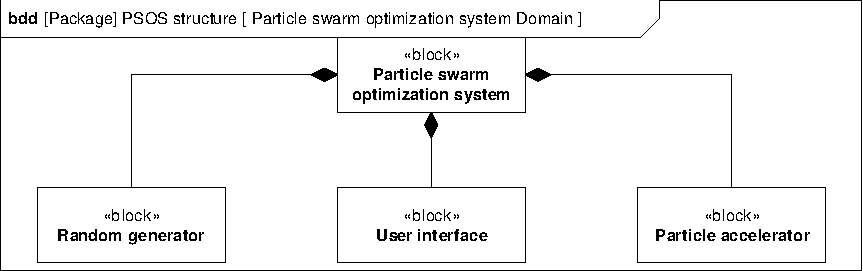
\includegraphics[width=0.8\linewidth]{diagram/bdd_particle_swarm_optimization_system.pdf}
	\caption{Block Definition Diagram}
	\label{fig:bdd}
\end{figure}

\textbf{Random Generator:}\\
The Random Generator block is needed, to generate random seeds for use in the particle swarm algorithm.\\

\textbf{User Interface:}\\
The User Interface block needs core functionality to communicate with the system. It needs to be able to take inputs regarding the particle swarm algorithms variables and create a graphical representation of the results to the user, after a successful particle swarm analysis.\\

\textbf{Particle Accelerator:}\\
The Particle Accelerator block has the functionality to perform the particle swarm optimization algorithm. Variables for the algorithm, given by the user, are communicated via the User Interface block. The random seed for the algorithm is given by the Random Generator block.

\subsubsection{Internal Block Diagram}


\begin{figure}[!h]
	\centering
	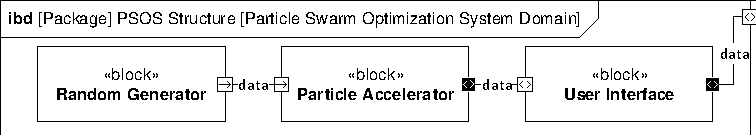
\includegraphics[width=0.8\linewidth]{diagram/ibd_particle_swarm_optimization_system.pdf}
	\caption{Internal Block Diagram}
	\label{fig:ibd}
\end{figure}

\subsection{Behavior}

\subsubsection{Activity Diagram}

\subsubsection{Sequence Diagram}






